%%%%%%%%%%%%%%%%%%%%%%%%%%%%%%%%%%%%%%%%%
% Journal Article
% LaTeX Template
% Version 1.4 (15/5/16)
%
% This template has been downloaded from:
% http://www.LaTeXTemplates.com
%
% Original author:
% Frits Wenneker (http://www.howtotex.com) with extensive modifications by
% Vel (vel@LaTeXTemplates.com)
%
% License:
% CC BY-NC-SA 3.0 (http://creativecommons.org/licenses/by-nc-sa/3.0/)
%
%%%%%%%%%%%%%%%%%%%%%%%%%%%%%%%%%%%%%%%%%

%----------------------------------------------------------------------------------------
%	PACKAGES AND OTHER DOCUMENT CONFIGURATIONS
%----------------------------------------------------------------------------------------

%\documentclass{article}
%\documentclass[oneside,twocolumn]{article}
\documentclass[oneside,onecolumn]{article}

\usepackage{blindtext} % Package to generate dummy text throughout this template 
\usepackage{multicol}
\usepackage[sc]{mathpazo} % Use the Palatino font
\usepackage[T1]{fontenc} % Use 8-bit encoding that has 256 glyphs
\linespread{1.05} % Line spacing - Palatino needs more space between lines
\usepackage{microtype} % Slightly tweak font spacing for aesthetics

%\usepackage[english]{babel} % Language hyphenation and typographical rules
\usepackage[spanish]{babel}
\usepackage[hmarginratio=1:1,top=32mm,columnsep=20pt]{geometry} % Document margins
\usepackage[hang, small,labelfont=bf,up,textfont=it,up]{caption} % Custom captions under/above floats in tables or figures
\usepackage{booktabs} % Horizontal rules in tables

\usepackage{lettrine} % The lettrine is the first enlarged letter at the beginning of the text

\usepackage{listings} % Required for insertion of code

\usepackage{enumitem} % Customized lists
\setlist[itemize]{noitemsep} % Make itemize lists more compact

\usepackage{abstract} % Allows abstract customization
\renewcommand{\abstractnamefont}{\normalfont\bfseries} % Set the "Abstract" text to bold
\renewcommand{\abstracttextfont}{\normalfont\small\itshape} % Set the abstract itself to small italic text

\usepackage{titlesec} % Allows customization of titles
\renewcommand\thesection{\Roman{section}} % Roman numerals for the sections
\renewcommand\thesubsection{\roman{subsection}} % roman numerals for subsections
\titleformat{\section}[block]{\large\scshape\centering}{\thesection.}{1em}{} % Change the look of the section titles
\titleformat{\subsection}[block]{\large}{\thesubsection.}{1em}{} % Change the look of the section titles

\usepackage{fancyhdr} % Headers and footers
\pagestyle{fancy} % All pages have headers and footers
\fancyhead{} % Blank out the default header
\fancyfoot{} % Blank out the default footer
%\fancyhead[C]{Running title $\bullet$ May 2016 $\bullet$ Vol. XXI, No. 1} % Custom header text
\fancyfoot[RO,LE]{\thepage} % Custom footer text

\usepackage{titling} % Customizing the title section

\usepackage{hyperref} % For hyperlinks in the PDF

\usepackage{listings}
\usepackage{algorithm2e}
\usepackage{graphicx}
\usepackage[dvipsnames]{xcolor}
\definecolor{codegreen}{rgb}{0,0.6,0}
\definecolor{codegray}{rgb}{0.5,0.5,0.5}
\definecolor{codepurple}{rgb}{0.58,0,0.82}
\definecolor{backcolour}{rgb}{1,1,1}
\lstdefinestyle{mystyle}{
    backgroundcolor=\color{backcolour},   
    commentstyle=\color{codegreen},
    keywordstyle=\color{magenta},
    numberstyle=\tiny\color{codegray},
    stringstyle=\color{codepurple},
    basicstyle=\ttfamily\footnotesize,
    breakatwhitespace=false,         
    breaklines=true,                 
    captionpos=b,                    
    keepspaces=true,                 
    numbers=left,                    
    numbersep=5pt,                  
    showspaces=false,                
    showstringspaces=false,
    showtabs=false,                  
    tabsize=2
}
\renewcommand{\lstlistingname}{Código}% Listing -> Algorithm
\lstset{style=mystyle}

\usepackage[utf8]{inputenc} % Required for inputting international characters
\usepackage[T1]{fontenc} % Output font encoding for international characters
\usepackage{multirow}
\usepackage{amsmath}
%----------------------------------------------------------------------------------------
%	TITLE SECTION
%----------------------------------------------------------------------------------------

\setlength{\droptitle}{-4\baselineskip} % Move the title up

\pretitle{\begin{center}\Huge\bfseries} % Article title formatting
\posttitle{\end{center}} % Article title closing formatting
\title{Edge Bandwidth} % Article title
\author{%
\textsc{Luis Alberto Ballado Aradias} \\%\thanks{A thank you or further information} \\[1ex] % Your name
\normalsize Cinvestav Unidad Tamaulipas \\ % Your institution
\normalsize luis.ballado@cinvestav.mx % Your email address
%\and % Uncomment if 2 authors are required, duplicate these 4 lines if more
%\textsc{Jane Smith}\thanks{Corresponding author} \\[1ex] % Second author's name
%\normalsize University of Utah \\ % Second author's institution
%\normalsize \href{mailto:jane@smith.com}{jane@smith.com} % Second author's email address
}
\date{\today} % Leave empty to omit a date

%\renewcommand{\maketitlehookd}{%
%  \begin{abstract}
%    \noindent El presente trabajo describe la implementación del algoritmo bug2, con ayuda de los módulos desarrollados anteriormente como el de odometría para un robot móvil de tipo diferencial y su implementación bajo el lenguaje NXC (Not eXactly C).\\
%    El algoritmo Bug2 es un algoritmo de navegación en robótica que se utiliza para que un robot encuentre su camino hacia un destino en un ambiente desconocido, sin la necesidad de utilizar un mapa previamente construido. Este algoritmo se basa en la idea de que el robot puede seguir la pared del obstáculo que se encuentra en su camino hacia el destino.
%  \end{abstract}
%}

%----------------------------------------------------------------------------------------

\begin{document}

% Print the title
\maketitle

%----------------------------------------------------------------------------------------
%	ARTICLE CONTENTS
%----------------------------------------------------------------------------------------
\section{Introducción}

\lettrine[nindent=0em,lines=3]{E}l cálculo del Edge Bandwidth es un problema importante en redes de comunicaciones para determinar la capacidad de transferencia de datos entre dos nodos en la red.\\

El max bandwidth se refiere a la cantidad máxima de datos que pueden transferirse por segundo a través de una conexión entre dos nodos de la red. El cálculo puede ser de gran utilidad en diferentes situaciones como identificar cuellos de botella en la red que puedan estar afectando el rendimiento, o para planificar la expansión de una infraestructura de res. Además, es de gran utilidad en aplicaciones de transmisión de video en tiempo real, la transferencia de archivos de gran tamaño, solo por mencionar algunas aplicaciones a este problema.\\

El cálculo del \textbf{edge-bandwidth} de un grafo es el mínimo entre todos los posibles costos de aristas de la máxima diferencia entre dos aritas adyacentes. 

\begin{center}
  \[B_f(G) = max{|f(u)-f(v)|: uv \in E}\]
\end{center}

\subsection{Objetivo del proyecto}

Partiendo de ellos, se busca crear una estructura de datos que nos ayude a realizar un cálculo que, tal vez no sea el óptimo, buscar reducir los tiempos de ejecución haciendo uso de estructuras de datos capaces de poder tomar ventaja de los ciclos necesarios para poder trabajar en el problema

\subsection{Comparativa de eficiencia de algoritmos}



\newpage
\section{Pseudocódigos}

\SetKwComment{Comment}{/* }{ */}

\begin{algorithm}
\caption{Evaluación Secuencial}\label{alg:one}
\For{para i = 0 en lista de aristasAdyacentes}{
  $maxDif \gets 0$
  difAbs = abs(solucion[primer elemento respecto a la lista de aristasAdyacentes] - solucion[segundo elemento respecto a la lista de aristasAdyacentes]);\\
  \If{difAbs > maxDif}{
    $maxDif \gets difAbs$ \Comment*[r]{ir guardando el máximo}
  }
  \Return maxDif;
}
\end{algorithm}


\SetKwComment{Comment}{/* }{ */}

\begin{algorithm}
\caption{Evaluación Incremental}\label{alg:two}

\For{para i = 0 en lista de aristasAdyacentes[u].vecinos.size()}{
  $maxDif1 \gets 0$
  difAbs = abs(solucion[aristasAdyacentes[aristas\_v[u].positions[i]].first] - solucion[aristasAdyacentes[aristas\_v[u].positions[i]].second]); \Comment*[r]{se itera respecto a los vecinos que tenga u}
  \If{difAbs > maxDif}{
    $maxDif1 \gets difAbs$ \Comment*[r]{ir guardando el máximo}
  }
}

\For{para i = 0 en lista de aristasAdyacentes[v].vecinos.size()}{
  $maxDif2 \gets 0$
  difAbs = abs(solucion[aristasAdyacentes[aristas\_v[u].positions[i]].first] - solucion[aristasAdyacentes[aristas\_v[u].positions[i]].second]); \Comment*[r]{se itera respecto a los vecinos que tenga v}
  \If{difAbs > maxDif}{
    $maxDif2 \gets difAbs$ \Comment*[r]{ir guardando el máximo}
  }
}

\Return max(maxDif1,maxDif2);

\end{algorithm}


\newpage
\section{Análisis matemático}

Nuestro primer algoritmo de evaluación secuencial tiene que recorrer los n elementos que contenga el la lista de aristas adyacentes, siendo una complejidad lineal del orden $O(n)$. Nuestro segundo algoritmo de evaluación incremental al conocer el indice, se itera respecto a los vecinos que pueda tener. Se realiza tanto para u y v, con una complejidad constante respecto a la cardinalidad de ambos $O(u+v)$ . Pero depende de la cardinalidad que pueda tener y variando de grafo en grafo.

\section{Experimentación y Resultados}

La evaluación secuencial se hace respecto a la cardinalidad del vector de aristas adyacentes.\\

Para evitar el barrido en los cambios de etiquetado (swap(u,v)) se propone aprovechar la primera corrida para crear un vector que almacenará un objeto de tipo EdgeInfo que contiene el índice (consecutivo usado para hacer referecia a él). De esta forma se logra evitar recorrer nuevamente para el cálculo de un nuevo \textbf{Edge Bandwidth}, reduciendo el cálculo a la cardinalidad del vector de aristas vecinas de los elementos a intercambiar en el swap(u,v) w parejas de u; p parejas de v.


De esta manera el vector se pobla al momento de ir formando la lista de adyacencia, y se agregarán los indices vecinos al iterar la lista de adyacencia formando los pares.

\newpage

\begin{figure}[h]
  \centering
  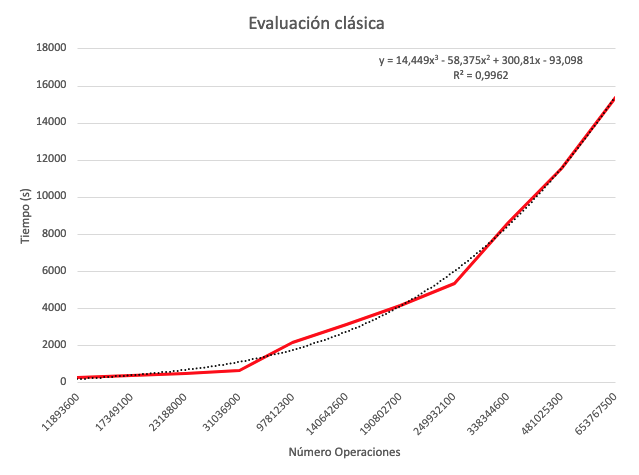
\includegraphics[scale=0.52]{graficos/eval_clasic.png}
  \caption{Gráfico de resultados Evaluación Clásica}
\end{figure}

\begin{table}[h]
  \caption{Tabla de resultados con la evaluación clásica}
  \centering
  \begin{tabular}{|l|l|l|l|}
    \hline
    Problema  & Evaluación & Llamadas  & Tiempo (ms) \\ \hline
    n100 p0,5 & Clásica    & 11893600  & 269,86      \\ \hline
    n100 p0,6 & Clásica    & 17349100  & 381,1       \\ \hline
    n100 p0,7 & Clásica    & 23188000  & 502,8       \\ \hline
    n100 p0,8 & Clásica    & 31036900  & 685,73      \\ \hline
    n200 p0,5 & Clásica    & 97812300  & 2187,36     \\ \hline
    n200 p0,6 & Clásica    & 140642600 & 3125,26     \\ \hline
    n200 p0,7 & Clásica    & 190802700 & 4181,23     \\ \hline
    n200 p0,8 & Clásica    & 249932100 & 5344,96     \\ \hline
    n300 p0,5 & Clásica    & 338344600 & 8573,06     \\ \hline
    n300 p0,6 & Clásica    & 481025300 & 11572,93    \\ \hline
    n300 p0,7 & Clásica    & 653767500 & 15408,46    \\ \hline
  \end{tabular}
\end{table}

\newpage

\begin{figure}[h]
  \centering
  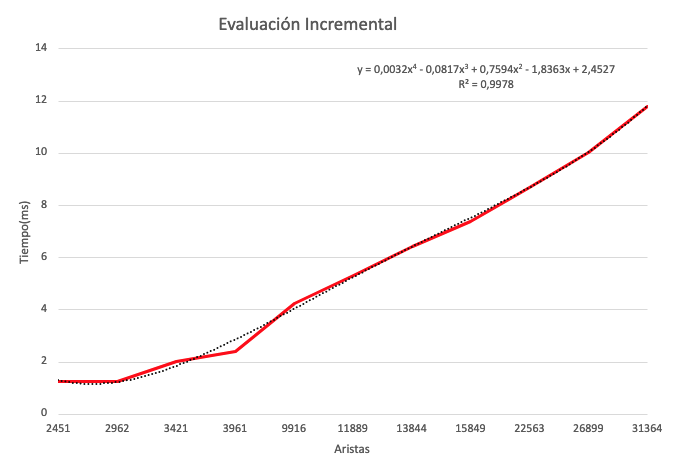
\includegraphics[scale=0.52]{graficos/eval_incr.png}
  \caption{Gráfico de resultados Evaluación Incremental}
\end{figure}

\begin{table}[h]
  \caption{Tabla de resultados con la evaluación incremental}
  \centering
  \begin{tabular}{|l|l|l|l|}
    \hline
    Problema  & Evaluación  & Llamadas & Tiempo (ms) \\ \hline
    n100 p0,5 & Incremental & 192,66   & 1,26        \\ \hline
    n100 p0,6 & Incremental & 236,1    & 1,26        \\ \hline
    n100 p0,7 & Incremental & 271,56   & 2,03        \\ \hline
    n100 p0,8 & Incremental & 311,46   & 2,4         \\ \hline
    n200 p0,5 & Incremental & 401,033  & 4,23        \\ \hline
    n200 p0,6 & Incremental & 478,86   & 5,3         \\ \hline
    n200 p0,7 & Incremental & 550,13   & 6,43        \\ \hline
    n200 p0,8 & Incremental & 630,96   & 7,4         \\ \hline
    n300 p0,5 & Incremental & 593,96   & 8,7         \\ \hline
    n300 p0,6 & Incremental & 718,53   & 10,03       \\ \hline
    n300 p0,7 & Incremental & 838,866  & 11,8        \\ \hline
  \end{tabular}
\end{table}



Considerando los resultados de las graficas déspues de experimentar la corrida con grafos bipartitos completos, el comportamiento es del orden polinomial. Esto es debido al aumento del problema en cada ejecución.\\

En la segunda grafica se observa la tendencia lineal de la evaluación incremental, no obstante no podemos considerar que una es mejor que la otra. Cabe señalar que no atacamos el problema \textbf{max bandwidth} de manera de busca el óptimo y sólo realizamos el intercambio de posiciones evitando recalcular toda la lista de pares de aristas adyacentes. Pero puede ser piedra angular para aplicarlo a una metaheurística de manera de ir encontrando una mejor solución respecto a los objetivos del \textbf{max bandwidth}


\newpage
\section{Aprendizajes}

Al cursar el curso de Análisis y diseño de algortimos, logré acercarme al análisis de grafos más allá de lo visto en matemáticas discretas. El poder manipularlo, explorarlo y lograr obtener una herramienta poderosa como lo es una estructura y representación de un grafo. Es bien sabido que varios problemas en nuestra vida cotidiana se pueden llegar a representar con grafos. Tal es así que traté de llevarlo a mis otras materias, así como el empujón que siempre quise tener para comenzar a programar en C++. Salirme de mi zona de confort, y ampliar mis conocimientos en lenguajes que no pasan de moda y altamente portable.\\

Aunque es un hecho que no repartí mi tiempo de forma equitativa entre todas las materias, logré llevar los conocimientos de clase a los demás proyectos como en computo paralelo, desarrollando el proyecto en C++ y cambiando mi paradigma a utilizar algoritmos vistos en clase.\\

Se muy bien que mi desempeño pudó ser mejor y a pesar de los altibajos logré con ayuda del Dr. Eduardo Tello a quién agradezco por sus palabras de aliento cuando imaginaba que mi proyecto de estudiar una Maestria en Ciencias se venía abajo. Eso ya no es un problema para mí, ya que considero que los conocimientos adquiridos este cuatrimestre serán de gran ayuda para el desarrollo de códigos adaptables y modulares cuando me toque regresar a la vida laboral.\\

No espero obtener una buena calificación, pero reconozco el esfuerzo que dedique en la materia con la esperanza de obtener una nota mínima aprobatoria.

%------------------------------------------------
\section{Conclusiones}

Como se mencionó en clases, la algorítmica es reconocida como la pieda angular de las ciencias computacionales. El saber de ellas, y aplicarlas es de suma importancia para el desarrollo de códigos limpios.\\

El manejo de abstracciones de clases, las estructuras de datos para generar algoritmos eficientes es de suma importancia. Un ejemplo de ello fué en el presente trabajo donde se logró reducir considerablemente el tiempo de ejecución con simples estructuras aprovechando los ciclos donde se forma la información, para así hacer uso de ellos en pasos posteriores, aunque pueda afectar en el crecimiento espacial, es algo con el que podemos llegar a lidiar. Quitandonos así de tiempos de ejecuciones altos, logrando eficienciar nuestro código.

%----------------------------------------------------------------------------------------
%	REFERENCE LIST
%----------------------------------------------------------------------------------------
\newpage
\begin{thebibliography}{0} % Bibliography - this is intentionally simple in this template
\bibitem{calamoneri} New results on edge-bandwidth, Theoretical Computer Science, Tiziana Calamoneri(a), Annalisa Massini(a), Imrich Vrto(b), (a) Computer Science Department, University of Rome, (b) Institute of Mathematics, Slovak Academy of Sciences, Department of Informatics, Bratislava, 2003
\bibitem{balogh} On the edge-bandwidth of graph products, Theoretical Computer Science, József Balog(a), Dhruv Mubayi(b), András Pluhár(c), (a) Department of Mathematical Sciences, The Ohio State University, Columbus OH, USA, (b) Department of Mathematics, Statistics, and Computer Science, University of Illinois, Chicago IL, USA, (c) Department of Computer Science, University of Szeged, Hungary, 2006
    
\end{thebibliography}

%----------------------------------------------------------------------------------------

\end{document}
